\section{Metodologia}

\begin{frame}{Arquitetura geral do SiameseFWI}
	\begin{columns}[T]
		\column{0.58\textwidth}
		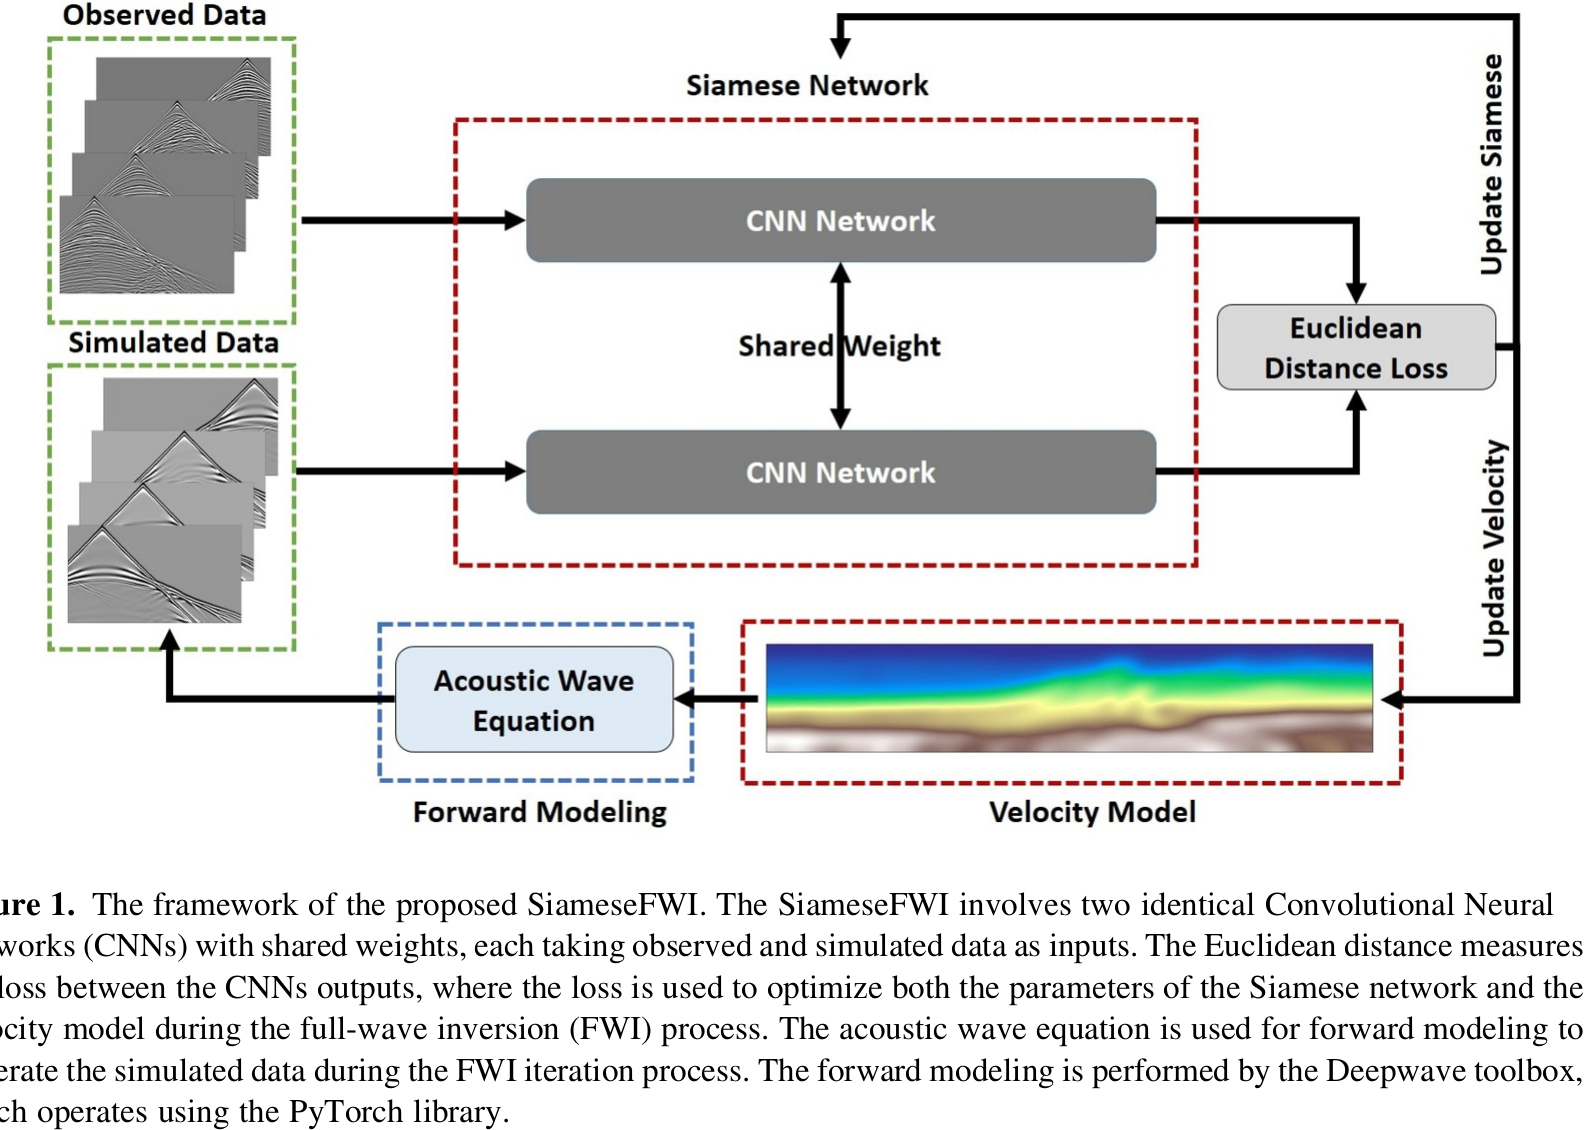
\includegraphics[width=\textwidth]{figuras/paper/fig1_framework}
		\column{0.42\textwidth}
		\begin{itemize}
			\footnotesize
			\setlength{\itemsep}{4pt}
			\item Duas CNNs idênticas, com pesos compartilhados, extraem \textit{features} do dado observado e do dado simulado.
			\item A distância Euclidiana entre as \textit{features} é a perda do SiameseFWI.
			\item Essa perda atualiza, ao mesmo tempo, os pesos da rede siamesa \textbf{e} o modelo de velocidade.
		\end{itemize}
	\end{columns}
\end{frame}

\begin{frame}{Teoria: modelagem direta e função de perda}
	\small
	\setlength{\abovedisplayskip}{4pt}
	\setlength{\belowdisplayskip}{4pt}
	Equação de onda acústica 2D, usada para gerar o dado simulado a cada iteração:
	\begin{equation}
		\nabla^2 p(r,t) = \frac{1}{v^2(r)} \frac{\partial^2 p(r,t)}{\partial t^2} + s(r,t)\,\delta(r - r_s)
	\end{equation}
	Distância Euclidiana entre as \textit{features} extraídas pela rede siamesa, usada como função de perda:
	\begin{equation}
		E = \sqrt{\sum_{i=0}^{n} \big(C(d_{obs}, \phi) - C(d_{sim}, \phi)\big)^2}
	\end{equation}
	\vspace{-0.2cm}
	\begin{itemize}
		\footnotesize
		\item $d_{obs}$ e $d_{sim}$: dado observado e simulado; $C$ e $\phi$: a CNN e seus parâmetros.
		\item Dois otimizadores Adam separados: um para o modelo de velocidade, outro para a rede siamesa.
	\end{itemize}
\end{frame}

\begin{frame}{A rede CNN da arquitetura siamesa}
	\begin{center}
		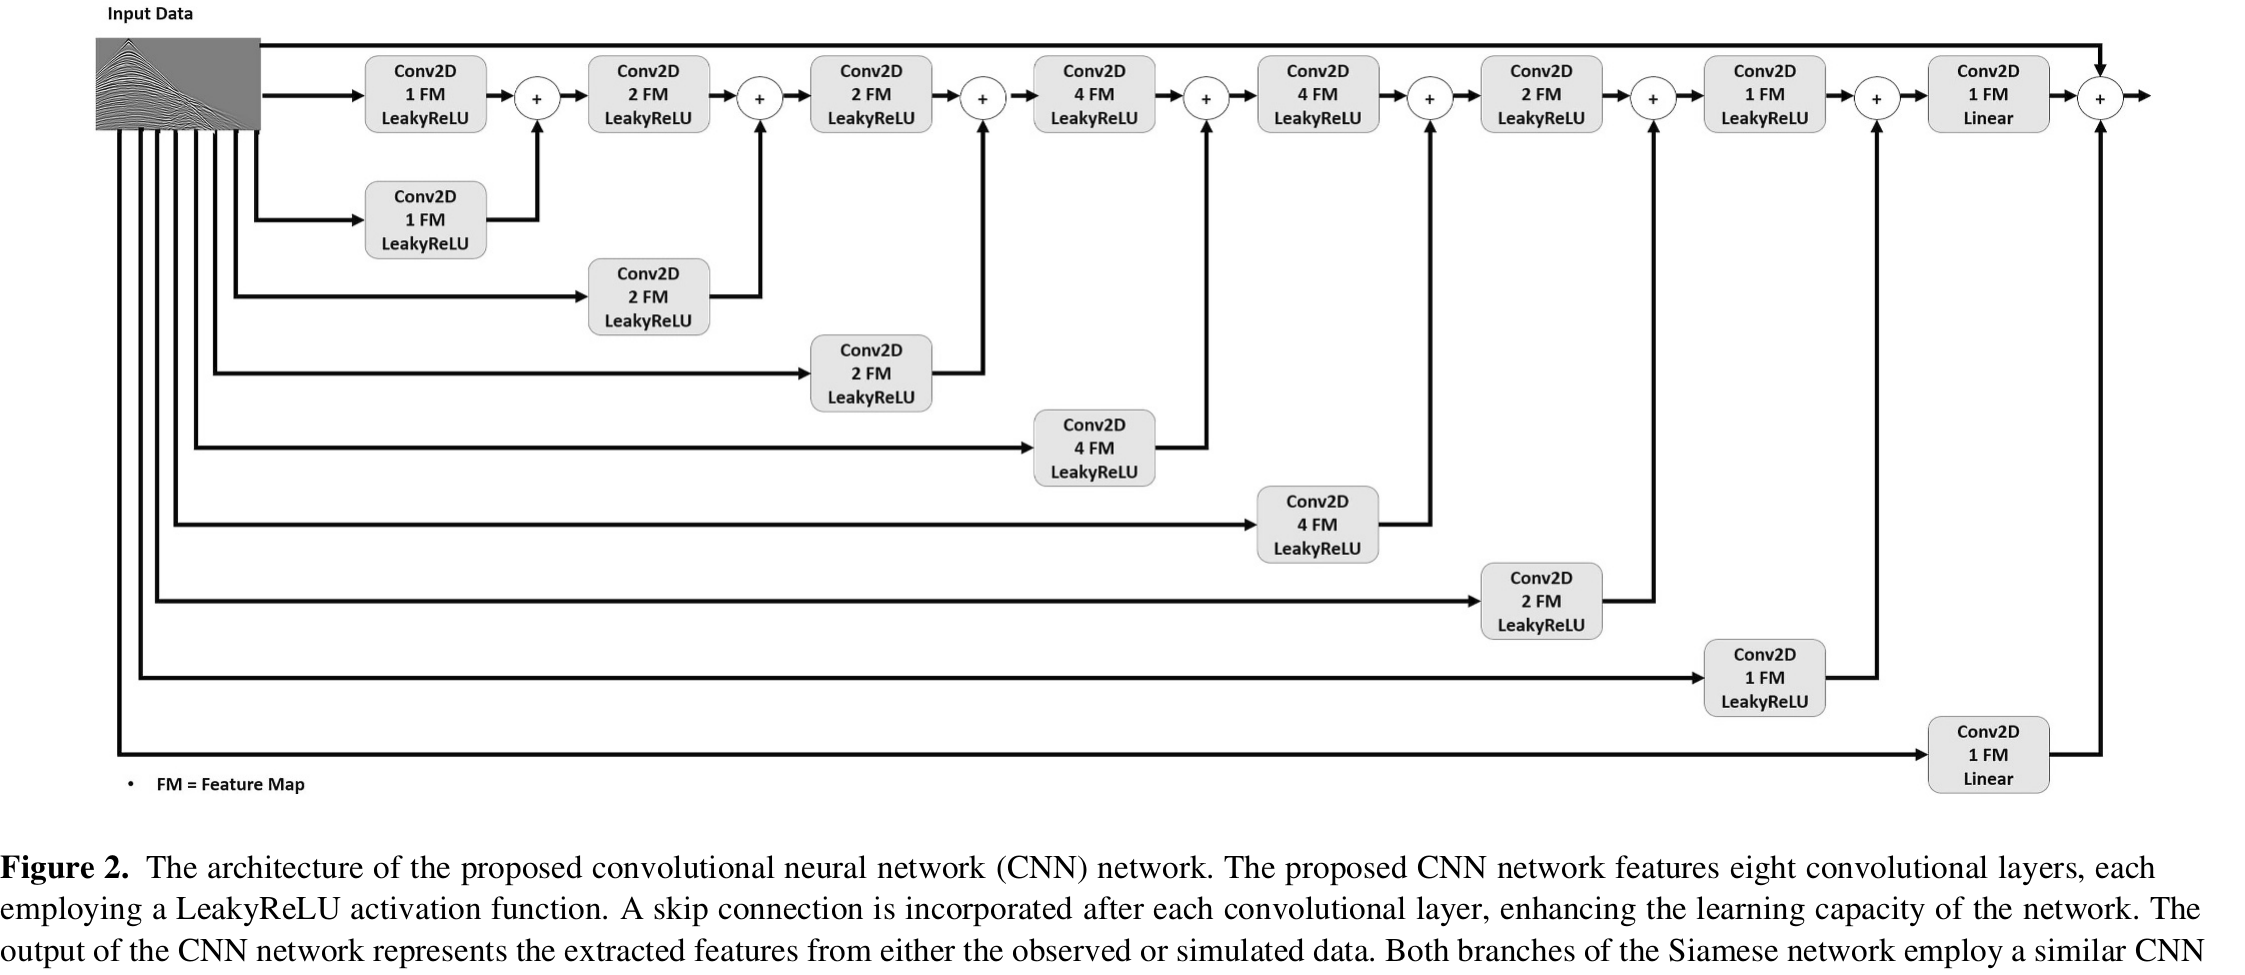
\includegraphics[width=0.95\textwidth]{figuras/paper/fig2_cnn}
	\end{center}
	\begin{itemize}
		\footnotesize
		\item 8 camadas convolucionais 3$\times$3 com LeakyReLU, exceto a última, linear.
		\item 8 conexões residuais (\textit{skip connections}), sem camada de \textit{pooling}: o tamanho espacial da entrada é preservado em toda a rede.
		\item Pesos inicializados aleatoriamente e otimizados ao longo do processo de FWI, sem pré-treinamento.
	\end{itemize}
\end{frame}
